%%% Template originaly created by Karol Kozioł (mail@karol-koziol.net) and modified for ShareLaTeX use

\documentclass[a4paper,11pt]{article}

\usepackage[T1]{fontenc}
\usepackage[utf8]{inputenc}
\usepackage{graphicx}
\usepackage{xcolor}
\usepackage[portuguese]{babel}

\renewcommand\familydefault{\sfdefault}
\usepackage{tgheros}
\usepackage[defaultmono]{droidmono}

\usepackage{amsmath,amssymb,amsthm,textcomp}
\usepackage{enumerate}
\usepackage{multicol}
\usepackage{tikz}

\usepackage{geometry}
\geometry{total={210mm,297mm},
left=25mm,right=25mm,%
bindingoffset=0mm, top=20mm,bottom=20mm}


\linespread{1.3}

\newcommand{\linia}{\rule{\linewidth}{0.5pt}}

% custom theorems if needed
\newtheoremstyle{mytheor}
    {1ex}{1ex}{\normalfont}{0pt}{\scshape}{.}{1ex}
    {{\thmname{#1 }}{\thmnumber{#2}}{\thmnote{ (#3)}}}

\theoremstyle{mytheor}
\newtheorem{defi}{Definition}

% my own titles
\makeatletter
\renewcommand{\maketitle}{
\begin{center}
\vspace{2ex}
{\huge \textsc{\@title}}
\vspace{1ex}
\\
\linia\\
\@author \hfill \@date
\vspace{4ex}
\end{center}
}
\makeatother
%%%

% custom footers and headers
\usepackage{fancyhdr}
\pagestyle{fancy}
\lhead{}
\chead{}
\rhead{}
\lfoot{PRC - MEI}
\cfoot{}
\rfoot{Page \thepage}
\renewcommand{\headrulewidth}{0pt}
\renewcommand{\footrulewidth}{0pt}
%

% code listing settings
\usepackage{listings}
\lstset{
    language=SPARQL,
    basicstyle=\ttfamily\scriptsize,
    aboveskip={1.0\baselineskip},
    belowskip={1.0\baselineskip},
    columns=fixed,
    extendedchars=true,
    breaklines=true,
    tabsize=4,
    prebreak=\raisebox{0ex}[0ex][0ex]{\ensuremath{\hookleftarrow}},
    frame=lines,
    showtabs=false,
    showspaces=false,
    showstringspaces=false,
    keywordstyle=\color[rgb]{0.627,0.126,0.941},
    commentstyle=\color[rgb]{0.133,0.545,0.133},
    stringstyle=\color[rgb]{01,0,0},
    numbers=left,
    numberstyle=\tiny,
    stepnumber=1,
    numbersep=10pt,
    captionpos=t,
    escapeinside={\%*}{*)}
}



%%%----------%%%----------%%%----------%%%----------%%%

\begin{document}

\title{Desenvolvimento de uma Ontologia }

\author{José Pereira PG 27748, Universidade do Minho}

\date{16/07/2015}

\maketitle

\section*{Introdução}
Uma ontologia é uma representação formal de conhecimento. Com ela é possível descrever universos complexos de uma forma relacional bastante simples. Neste documento, é descrita uma destas representações no contexto da computação. O domínio estudado é referente à plataforma concreta de comércio de vídeo jogos \textit{Steam}.
\subsection{Steam}
Atualmente a \textit{Steam} conta com aproximadamente 65 milhões de utilizadores ativos e tem médias de acesso diário de 6,6 milhões de contas em simultâneo. A plataforma também possuí um sistema de amigos, que permite ao utilizador manter uma rede de contactos, com os quais pode jogar, trocar itens, comunicar, etc.\\
Para esta tarefa, apenas foi considerada a componente de distribuição de jogos desta plataforma, não incluindo qualquer informação relativa a utilizadores.

\section{Objectivos}
Para construir o produto requerido, foi necessário atingir alguns objetivos mais gerais e que foram levantados à partida:
\begin{itemize}
\item Adquirir informação para povoamento da ontologia;
\item Esquematizar o domínio de conhecimento de acordo com os dados aglomerados;
\item Explorar o potencial de aprendizagem da representação.
\newpage
\section{Abordagem}
Nesta secção é descrito o processo de construção da ontologia em detalhe. No percurso do desenvolvimento foram utilizadas as ferramentas:
\begin{itemize}
\item \textit{Scrapy} - Ferramenta que implementa uma solução de \textit{web crawling\footnote{Parsing de conteúdo HTML web para extração de informação.}} em \textit{Python};
\item \textit{XSLT} - Linguagem de marcação que define a apresentação de documentos \textit{XML};
\item \textit{Protégé} - Plataforma \textit{open-source} para desenvolvimento e manipulação de modelos de domínio.
\end{itemize}

\subsection{Captura de informação relevante}
O estudo de casos concretos e reais enriquece claramente o processo, daí a escolha de um domínio fiel. Para isto, e depois de alguma análise foi estipulado que a informação trabalhada seria obtida através das páginas HTML públicas destinadas ao comércio de jogos.
Para capturar tal informação, recorreu-se a uma ferramenta baseada em \textit{web crawling}. 

\lstset{
    language=Python,
    basicstyle=\ttfamily\scriptsize,
    aboveskip={1.0\baselineskip},
    belowskip={1.0\baselineskip},
    columns=fixed,
    extendedchars=true,
    breaklines=true,
    tabsize=4,
    prebreak=\raisebox{0ex}[0ex][0ex]{\ensuremath{\hookleftarrow}},
    frame=lines,
    showtabs=false,
    showspaces=false,
    showstringspaces=false,
    keywordstyle=\color[rgb]{0.627,0.126,0.941},
    commentstyle=\color[rgb]{0.133,0.545,0.133},
    stringstyle=\color[rgb]{01,0,0},
    numbers=left,
    numberstyle=\tiny,
    stepnumber=1,
    numbersep=10pt,
    captionpos=t,
    escapeinside={\%*}{*)}
}

\begin{lstlisting}[label={stub:first},caption=Lista de \textit{URLs} iniciais ao qual será aplicado um parsing e domínio sob o qual é permitido navegar]
start_urls = ["http://store.steampowered.com/tag/pt/Desporto#p=0&tab=NewReleases",
                  "http://store.steampowered.com/genre/Free%20to%20Play/",
                  "http://store.steampowered.com/genre/Early%20Access/",
                  "http://store.steampowered.com/tag/pt/Aventura/#p=0&tab=NewReleases",
                  "http://store.steampowered.com/tag/pt/Casual/#p=0&tab=NewReleases",
                  "http://store.steampowered.com/tag/pt/Corridas/#p=0&tab=NewReleases",
                  "http://store.steampowered.com/tag/pt/Estrat%C3%A9gia/#p=0&tab=NewReleases",
                  "http://store.steampowered.com/tag/pt/Indie/#p=0&tab=NewReleases",
                  "http://store.steampowered.com/tag/pt/Multijogador%20em%20Massa/#p=0&tab=NewReleases",
                  "http://store.steampowered.com/tag/pt/RPG/#p=0&tab=NewReleases",
                  "http://store.steampowered.com/tag/pt/Simula%C3%A7%C3%A3o/#p=0&tab=NewReleases"
                  ]
    allowed_domains = ["store.steampowered.com"]
\end{lstlisting}
\newpage
\begin{lstlisting}[label={stub:second},caption=Parser que irá ser aplicado ao conjunto de páginas alojadas nos URL mencionados anteriormente. Aplicação recursiva nas páginas associadas aos links presentes nestas.]
def parse(self, response):
        for href in response.xpath("//a/@href[contains(.,'http://store.steampowered.com/app/')]"):
            app_url = re.compile("http://store.steampowered.com/app/(\d+)/")
            url = response.urljoin(href.extract())
            if app_url.match(url):
                app_id = app_url.search(url).group(1)
                if app_id not in self.visited_ids:
                    self.visited_ids.append(app_id)
                    more_like_url = 'http://store.steampowered.com/recommended/morelike/app/'+str(app_id)
                    yield scrapy.Request(url, callback=self.parse_dir_contents)
                    yield scrapy.Request(more_like_url, callback=self.parse)
                    yield scrapy.Request(url, callback=self.parse)

\end{lstlisting}

\begin{lstlisting}[label={stub:third},caption=Exemplo de captura do atributo $nome$ de cada jogo recorrendo a \textit{XPath} sobre a árvore \textit{HTML}.]
#NOME DO JOGO
        for res in response.xpath("//div[@class='apphub_AppName']").xpath("text()").extract():
            item['nome'] = res

\end{lstlisting}
\begin{lstlisting}[label={stub:third},caption=Comando que exercita o código acima descrito e produz um documento \textit{XML} resultante.]
>> scrapy crawl steam_ontologia –o resultado.xml
\end{lstlisting}

\subsection{A ontologia}
Baseado na informação disponível/obtida no processo acima descrito, estipulou-se que a ontologia seria composta por 6 classes com a disposição ilustrada na figura 1.

\begin{figure}[!htb]
     \centering
      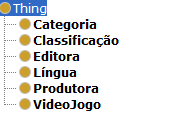
\includegraphics[scale=1]{classesontologia}
     \caption{Disposição das classes na ontologia}
     \label{fig1}
\end{figure} 
\newpage
\\

Para além das relações inter classe, existem diversas \textit{data properties} como exposto na figura 2.
\begin{figure}[!htb]
     \centering
      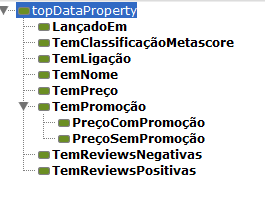
\includegraphics[scale=1]{data_properties}
     \caption{\textit{Data properties}}
     \label{fig2}
\end{figure} 
As relações entre classes são ilustradas na figura 3, como \textit{object properties}.
\begin{figure}[!htb]
     \centering
      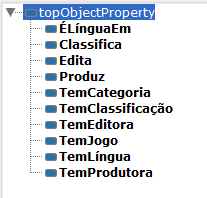
\includegraphics[scale=1]{object_properties}
     \caption{\textit{Object properties}}
     \label{fig3}
\end{figure} 
\subsection{De \textit{XML} para \textit{OWL}}
Adquiridos os dados e definida a ontologia, foi então necessário povoá-la. Para isto, utilizou-se um documento \textit{XSL} que reestruturou a informação extraída previamente e a converteu num documento \textit{OWL} apto a ser executado na ferramenta \textit{Protégé}.
\newpage
\subsection{Queries}
Para confirmar o sucesso do porte de informação, assim como a utilidade do produto construído, produziu-se a seguinte query \textit{SPARQL}:

\lstset{
    language=SPARQL,
    basicstyle=\ttfamily\scriptsize,
    aboveskip={1.0\baselineskip},
    belowskip={1.0\baselineskip},
    columns=fixed,
    extendedchars=true,
    breaklines=true,
    tabsize=4,
    prebreak=\raisebox{0ex}[0ex][0ex]{\ensuremath{\hookleftarrow}},
    frame=lines,
    showtabs=false,
    showspaces=false,
    showstringspaces=false,
    keywordstyle=\color[rgb]{0.627,0.126,0.941},
    commentstyle=\color[rgb]{0.133,0.545,0.133},
    stringstyle=\color[rgb]{01,0,0},
    numbers=left,
    numberstyle=\tiny,
    stepnumber=1,
    numbersep=10pt,
    captionpos=t,
    escapeinside={\%*}{*)}
}
\begin{lstlisting}[label={stub:forth},caption=Query SPARQL que identifica os cinco jogos mais baratos.]
PREFIX rdf: <http://www.w3.org/1999/02/22-rdf-syntax-ns#>
PREFIX owl: <http://www.w3.org/2002/07/owl#>
PREFIX rdfs: <http://www.w3.org/2000/01/rdf-schema#>
PREFIX xsd: <http://www.w3.org/2001/XMLSchema#>
PREFIX so: <http://www.semanticweb.org/jpereira/ontologies/2015/6/steam-ontologia#>


SELECT ?nome ?preco
WHERE {	?jogo rdf:type so:VideoJogo.
	?jogo so:TemNome ?nome.
	?jogo so:TemPreco ?preco.
}
ORDER BY ?preco
LIMIT 5
\end{lstlisting}
A figura 4, é o resultado de uma captura de ecrã sobre a página HTML correspondente ao item mais barato. Como se pode verificar, os valores coincidem.

\begin{figure}[!htb]
     \centering
      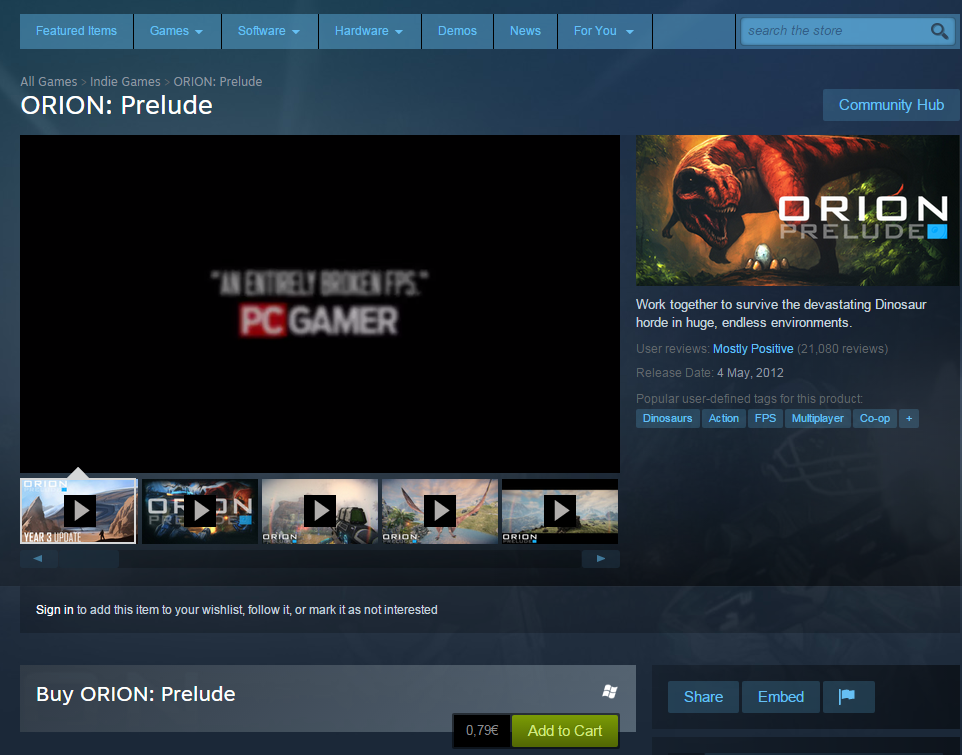
\includegraphics[scale=0.5]{mais_barato}
     \caption{Página HTML do jogo mais barato}
     \label{fig4}
\end{figure} 

\section{Conclusão}
Ontologias são conceitos muito poderosos e aplicáveis a qualquer contexto e que possibilitam inferir novo conhecimento útil baseado em regras algébricas simples. \\
Para além disto, foi enriquecedor manipular as ferramentas descritas, marcando referências para trabalho futuro.

\end{document}
